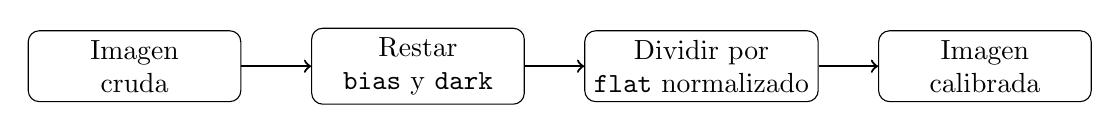
\begin{tikzpicture}[
  box/.style={draw,rounded corners,align=center,minimum width=2.7cm,minimum height=0.9cm},
  arrow/.style={->,thick}
]
  \node[box] (raw) at (0,0) {Imagen\\cruda};
  \node[box] (bias) at (3.6,0) {Restar\\\texttt{bias} y \texttt{dark}};
  \node[box] (flat) at (7.2,0) {Dividir por\\\texttt{flat} normalizado};
  \node[box] (clean) at (10.8,0) {Imagen\\calibrada};
  \draw[arrow] (raw) -- (bias);
  \draw[arrow] (bias) -- (flat);
  \draw[arrow] (flat) -- (clean);
\end{tikzpicture}